	\newpage
\section{Ogólne określenie wymagań projektu}		%1
%Ogólne określenie wymagań i zakresu programu (Czyli zleceniodawca określa wymagania programu) 

\subsection{Ogólny zarys wymagań}

Celem programu jest pełnienie funkcji odtwarzacza muzyki. Program będzie mógł skanować dany folder i jego podfoldery, a w nich zawarty pliki muzyczne i tworzyć na ich podstawie bibliotekę, zapisaną na dysku.  

\subsection{Wykorzystane czujniki}

Program ma na celu wykorzystanie trzech czujników, z którymi użytkownik będzie wchodził w interakcję. Zostaną użyte następujące:

\begin{itemize}
	\item Żyroskop - Interfejs programu będzie się zmieniał w zależności od orientacji urządzenia. 
	
	\item Wykrywacz odcisków palca - dostęp do programu powinien być ograniczony dla użytkowników mogących zweryfikować swój odcisk.

	\item Czujnik światła - Interfejs programu będzie mógł zmieniać swoje kolory w zależności od wykrytego poziomu światła na czujniku
\end{itemize}

\subsection{Zarys interfejsu}

\todo{Zmienić mockup widoku artystów. Dodać topbar i dać pola tekstowe w kafelki}

\begin{figure}[H]
	\centering
	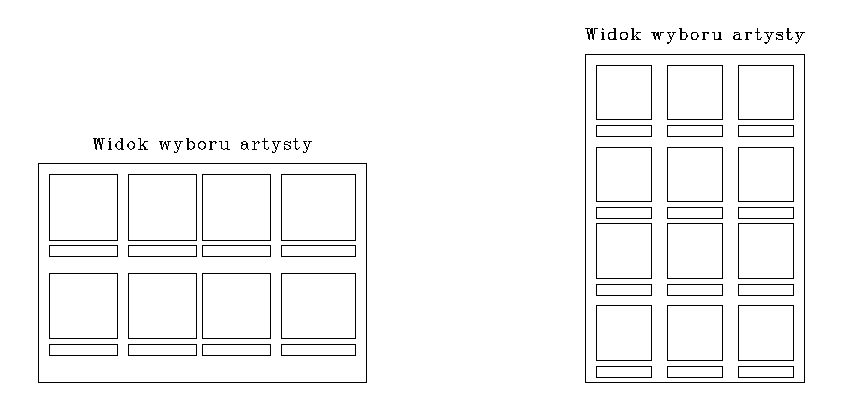
\includegraphics[width=1\linewidth]{images/mockup2_artysta}
	\caption{\centering{Mockup widoku biblioteki - listing wykonawców}}
	\label{fig:mockup2artysta}
\end{figure}

Widok wykonawców, jest przedstawiony na rysunku nr.~\ref{fig:mockup2artysta}. Ten widok będzie ekranem startowym aplikacji. Jako "Kafelki", zwracać będzie się dokument do ułożonych równomiernie na rysunku kwadratów. Na każdym z nich napisana będzie nazwa danego wykonawcy. Klikanie na jeden z nich przejdzie do widoku albumów danego wykonawcy.

\begin{figure}[H]
	\centering
	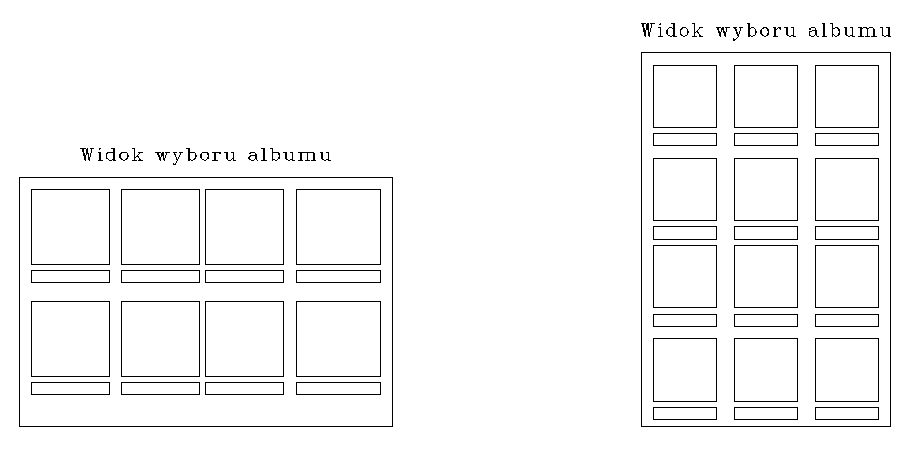
\includegraphics[width=1\linewidth]{images/mockup2_albumy}
	\caption{\centering{Mockup widoku albumów danego wykonawcy}}
	\label{fig:mockup2albumy}
\end{figure}

Widok albumów jest przedstawiony na rysunku nr.~\ref{fig:mockup2albumy}. Widok będzie podobny do widoku wykonawców. Różni się on tym, że na "kafelkach", będą pokazane zdjęcia poszczególnych albumów. Pod "kafelkami", znajdują się nazwy danych albumów.

\begin{figure}[H]
	\centering
	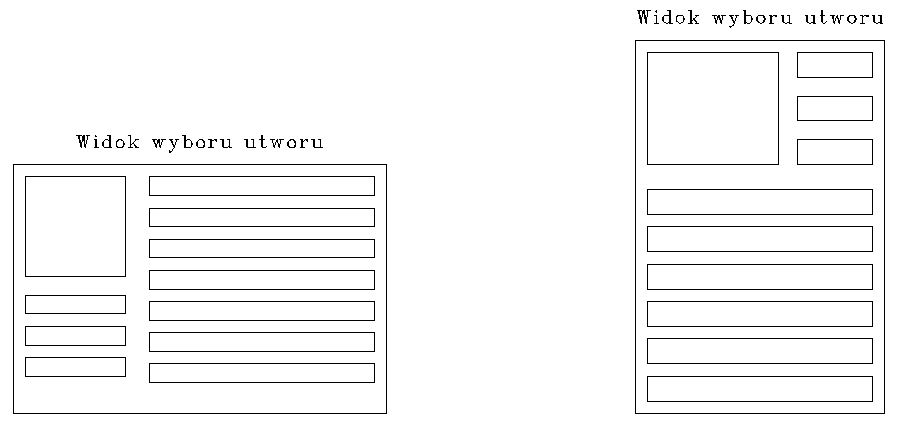
\includegraphics[width=1\linewidth]{images/mockup2_utwory}
	\caption{\centering{Mockup widoku wyboru utworu}}
	\label{fig:mockup2utwory}
\end{figure}


Rysunek nr.~\ref{fig:mockup2utwory} przedstawia ekran pokazujący się po wybraniu albumu. Po wejściu na jakiś album zaprezentowane zostaną zawarte w nim utwory. W lewym górnym kwadrat to zdjęcie danego albumu, a obok niego jest kilka informacji o albumie jak wykonawca, data, tytuł, w postaci tekstu. Dłuższe paski zawarte na dole to lista piosenek, w postaci przycisków z napisanymi, tytułami które można kliknąć, aby daną piosenkę włączyć.

\todo{To trzeba całe zmienić na nowe}
\begin{figure}[H]
	\centering
	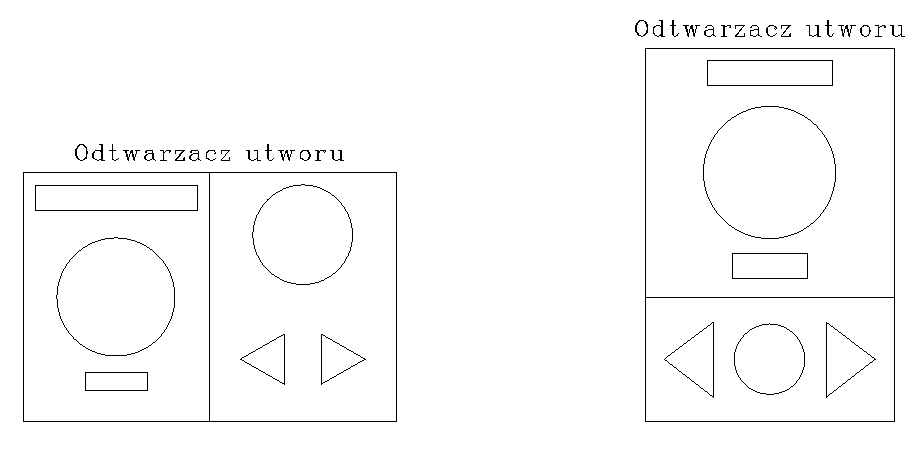
\includegraphics[width=1\linewidth]{images/mockup2_odtwarzacz}
	\caption{\centering{Mockup odtwarzacza}}
	\label{fig:mockup2odtwarzacz}
\end{figure}

Wygląd interfejsu odtwarzacza został zaprezentowany na rysunku nr.\ref{fig:mockup2odtwarzacz}. Odtwarzacz będzie działał następująco: duże koło będzie stylizowane na płytę, gdzie wypełniona ona będzie obrazem albumu. Płyta ta będzie się kręcić w czasie gdy gra piosenka. Kąt płyty (od 0\degree, do 360\degree) będzie określał jak duża część piosenki została odtworzona. Kąt ten będzie określony jeszcze niezdefiniowanym efektem graficznym. Prostokąty wokół płyty to tytuł piosenki, a na dole czas grania. Kółko i wokół niego trójkąty to przyciski odtwarzania - graj/pauza, następny, poprzedni.
